\section{Results}
\label{sec:casestudy}

We first summarize what replicated on held-out data and then answer the four research questions, each opening with its
answer. Table~\ref{tab:results} at the end lists every headline result with its evidence class.

\subsection{Held-out confirmation at a glance}
\label{sec:heldout}
\label{sec:v3}

On v2, 43 of 82 replicable claims confirm, 33 do not and 6 cannot be tested; on v3, 41 of 63 confirm and 3 cannot be
tested (Table~\ref{tab:v3}). The pattern is the same on both corpora: claims about accuracy, geometry, shared inputs,
atlas structure and failure prediction replicate, fewer than half of the single-feature causal claims do, and no claim
that two models share a causal effect replicates.

\begin{table}[!tb]
\centering
\footnotesize
\begin{tabular}{@{}lccc@{}}
\toprule
Registered claim type & v2 (971 series) & v3 (1{,}024 series) & Section \\
\midrule
Accuracy (Chronos-2 better on \texttt{mixture}) & 1/1 & 1/1 & \ref{sec:setup} \\
Peak-CKA pair & 1/1 & 1/1 & \ref{sec:rq2} \\
Concept transfer (shared inputs) & 20/20 & 20/20 & \ref{sec:rq2} \\
\quad same claims on 800 raw real windows & -- & 20/20 & \ref{sec:rq2} \\
Atlas structure & 2/2 & 2/2 & \ref{sec:rq2}, \ref{sec:rq3} \\
Single-model atlas concept & 1/1 & -- & \ref{sec:rq2} \\
Cross-model causal (atlas concepts; agreement) & 0/3; 0/6 & none registrable & \ref{sec:rq2} \\
Single-feature causal effect & 10/31 & 11/24 & \ref{sec:rq3} \\
Perturbation-profile agreement & 6/9 & 4/9 & \ref{sec:rq4} \\
Failure prediction from internals & 2/2 & 2/3 & \ref{sec:practical} \\
\midrule
Confirmed / replicable (not testable) & 43/82 (6) & 41/63 (3) & \\
\midrule
Window geometry, second sealed v3 split: & & & \\
\quad 21 pairs above null; mean understates 4 pairs & -- & 21/21; 4/4 & \ref{sec:rq2} \\
\bottomrule
\end{tabular}
\caption{Held-out confirmation on two independent corpora. Each cell is confirmed / tested; each claim type is one Holm
family. The external raw-window set and the second v3 split (512 of its 2{,}863 series used) are not counted in the
totals (\fid{CA-11}, \fid{CA-12}).}
\label{tab:v3}
\end{table}

\begin{figure}[!tb]
\centering
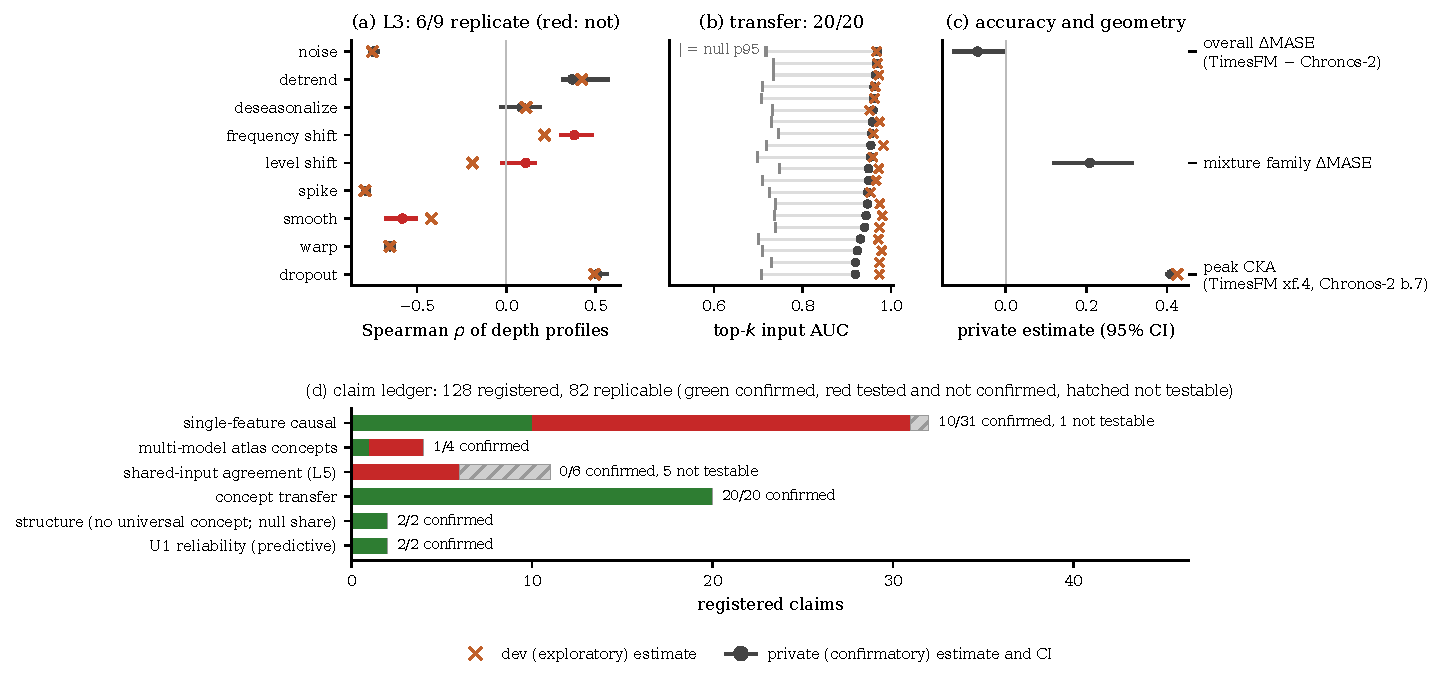
\includegraphics[width=\textwidth]{figures/heldout.pdf}
\caption{Claims re-tested on the sealed v2 private split (971 series; panel a uses 800 of them). (a) Per-corruption
depth-profile agreement, TimesFM vs.\ Chronos-2 (red: the dev value is not inside the private interval). (b) The 20
concept-transfer claims with private null 95th percentiles. (c) Accuracy and peak CKA; crosses are dev values, dots and
bars private values with 95\% series-bootstrap intervals. (d) Registered concept claims by type: confirmed, tested and
not confirmed, and not testable (the one confirmed atlas claim is single-model). Source:
\texttt{confirm/confirmation.json}.}
\label{fig:heldout}
\end{figure}

\subsection{RQ1: Which forecast-relevant concepts do TSFMs learn?}
\label{sec:rq1}

\textbf{Answer.} In six of the seven models, SAE features exist whose removal moves the forecast more than removing a
random decoded direction of the same size. They act mostly on forecast level and seasonality and form a graded continuum
rather than discrete units. Against random directions drawn from the activation distribution, few single features stand
out.

\paragraph{Causal features beyond isotropic directions.} Of the 56 target layers, 55 pass both reach controls; in
Chronos-2's final block the head reads placeholder tokens that a context patch never reaches (\fid{DE-03}). Across the
55 targets, 442 feature-channel cells clear the profile-matched null where the empirical chance rate predicts 178.75
(2.47 times chance). The ratio ranges from 1.64 (Chronos-T5-Base) to 5.70 (Chronos-Bolt) for six models; for Timer it is
1.02, although its layers do reach the forecast (\fid{PM-17}). Target by target, 22 of 55 targets clear significantly
more cells than chance (Benjamini--Hochberg at 0.05), at least two in every model except Timer. In all, 194 features clear
at least one channel, against at most 144.95 expected if channels were independent.

\paragraph{The effects concern level and seasonality.} Nine effect families tile the causal features
(Figure~\ref{fig:families}). The two largest act on level: \emph{level raisers} (45 features) and \emph{level lowerers}
(44), together 89 of the 192 assigned features. \emph{Seasonality dampeners} (25) and \emph{amplifiers} (19) follow;
three mixed-effect families (14, 13 and 11), \emph{trend boosters} (11) and \emph{volatility dampeners} (10) are smaller.

\begin{figure}[!tb]
\centering
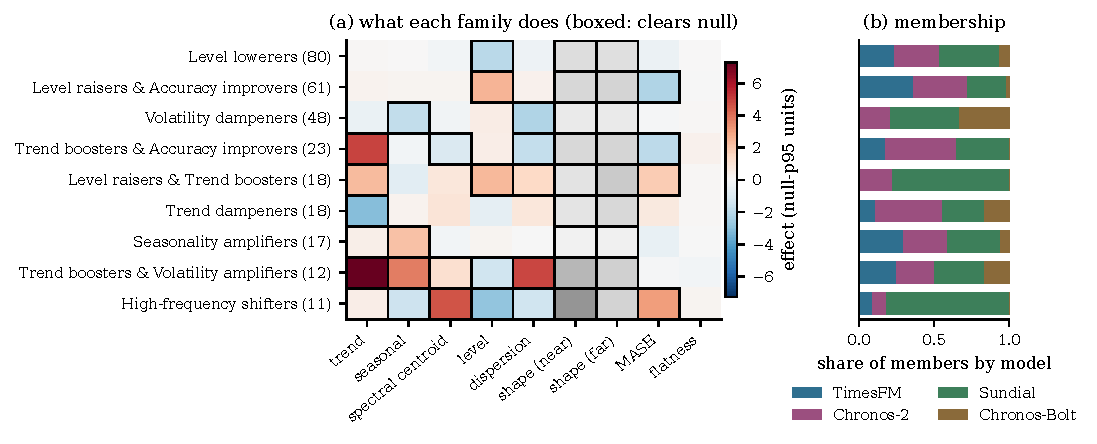
\includegraphics[width=\textwidth]{figures/families.pdf}
\caption{The nine causal-effect families. (a) Family centroid in null units, signed as what the feature
\emph{does} (red raises, blue lowers; boxed cells clear the null; shape distances unsigned, gray). (b)
Membership by model. Source: \texttt{sae/concept\_families.json}.}
\label{fig:families}
\end{figure}

\paragraph{The effects form a continuum.} Within a layer, 50 of 56 targets are non-modular; the 10 per-target concepts
that exist sit on 5 targets, 4 of them on Timer targets whose clear rate is at chance. The strict atlas assigns 35 of the
194 features to 11 concepts, more structure than a column-shuffle null produces (null 95th percentile 5.05 concepts;
assigned fraction 0.180 against 0.088; $p=0.005$) but covering few features. The families cover 192 of 194 features but do
not beat the shuffle null in number ($p=0.68$) or coverage ($p=0.23$), and the silhouette is 0.25--0.32 for every cut
from 6 to 16 families. The effect vectors are not low-dimensional (participation ratio 5.58 of 9 channels on v3;
\fid{MN-07}), so the absence of discrete families is not a lack of variation. The families are a vocabulary for reading
the effects, not discovered units.

\paragraph{Against on-manifold directions, features stand out only modestly.} The v3 run scored every feature against
both nulls. Under the isotropic null, 238 of 967 scorable features clear at least one channel; under the
covariance-matched null, 91 do. Scoring each null draw as a pseudo-feature on all nine channels at once, which keeps the
dependence between channels, gives expected counts of 67.0 and 70.4, so features exceed chance 3.55-fold against
isotropic directions ($p=4\times10^{-86}$) but only 1.29-fold against on-manifold ones (Poisson-binomial $p=0.0045$).
Even so, 11 of the 24 registered single-feature claims replicate on new series (Section~\ref{sec:rq3}).

\paragraph{Effects under on-manifold interventions.} We re-ran the 91 v3 features that clear the on-manifold null under
three further interventions, each with the null matched to its removal: setting the feature to its corpus mean (mean
ablation), replacing it by its activation at the same token of another series on which it fires (resample ablation), and
subtracting its decoder contribution from the model's own activation rather than from the reconstruction (clean
ablation). Of the 91 features, 69 still clear under mean ablation, 58 of 90 scorable ones under resample ablation and 49
under clean ablation; 79 clear under at least one and 37 under all three. Mean and resample ablation keep the direction of
the effect (median cosine to zero ablation 0.997 and 0.991), clean ablation less so (0.919). Survival under mean ablation
depends on density: 56 of 62 sparse features survive but only 13 of 29 dense ones, for which the mean also adds the
feature where it is silent. Of 91 sampled non-clearing features, 1, 2 and 8 clear under the three interventions
(\fid{MP-10}). Most causal features keep an effect under some on-manifold intervention, but which single features clear
depends on the intervention, consistent with a graded continuum.

\paragraph{Alignment with generative factors is correlational.} After dead-feature revival, 154 of 10{,}240 TimesFM
features and 115 of 6{,}144 Chronos-T5-Base features correlate with a ground-truth generative field beyond a permutation
null; the strongest is intermittency ($\rho=0.881$; \fid{MP-06}). The alignment does not extend to mediation: moving the
generator parameter does not change a matched feature's forecast effect beyond chance (\fid{MN-17}).

\subsection{RQ2: Are concepts shared across architectures?}
\label{sec:rq2}

\textbf{Answer.} Whole-layer geometry is shared above chance by all 21 model pairs, held-out. Different architectures
select the same series for a concept, held-out on both corpora and on raw real windows, and the broad effect types recur
in every model. At a fine grain, however, concepts are organized by model, and the same causal effect on the same series
is detected only between two Chronos-family models.

\paragraph{Geometry is shared above chance.} With concatenated windows, peak CKA (the maximum over layer pairs) between
TimesFM and each other model is 0.358--0.635 on v2 and 0.375--0.712 on v3 (512 series each), and all 21 model pairs exceed
their shuffled-series null on both corpora ($p=0.001$, 1000 permutations; null 95th percentiles 0.003--0.51, highest for
pairs with Time-MoE). The layer pairs selected on v3 dev were registered and tested once on a fresh sealed split: all 21
exceed their nulls (Holm $p=0.021$), with TimesFM/Chronos-2 at 0.707 [0.679, 0.734] against 0.712 on dev. At the same
layers and series, averaging a window's tokens lowers TimesFM's CKA with Chronos-2, Chronos-T5-Base, Chronos-Bolt and
Sundial by 0.322, 0.433, 0.301 and 0.303 (each 95\% interval above 0.26; Holm $p=0.0008$; \fid{MN-38}). Pairs with Timer
change little, because its 96-step token has no within-window order to match. Stitching agrees: concatenating the source
window raises the mean gain over the input baseline at the 21 peak pairs from 0.498 to 0.554, most when TimesFM is
predicted (from Chronos-T5-Base, 0.307 to 0.788), and keeps the ranking of pairs (Spearman 0.92).

\paragraph{Similarity has no single meaning.} Different metrics rank the 21 pairs inconsistently (Kendall's $W=0.25$,
$p=0.0095$, over seven metrics of the v2 run with mean-pooled CKA; Figure~\ref{fig:similarity}). TimesFM/Chronos-2 is
the most similar pair by error agreement (0.948) but 15th by mean-pooled CKA, where Sundial/Chronos-Bolt ranks first
(0.927); with concatenated windows TimesFM/Chronos-2 rises to 9th on v2 and 7th on v3. Geometry also does not reflect
lineage: an untrained pair scores higher than a trained, related pair (\fid{MN-01}). The report therefore never pools
similarity metrics into one score and reads CKA only against shuffled-series nulls.

\begin{figure}[!tb]
\centering
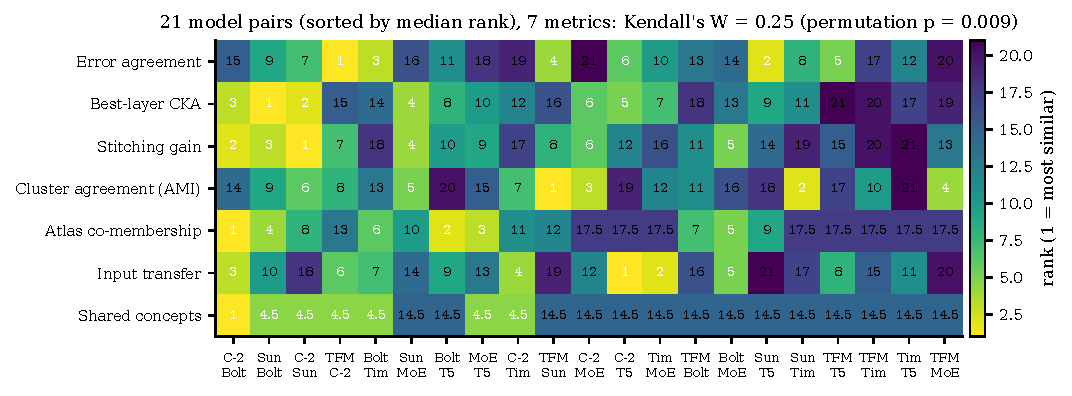
\includegraphics[width=\textwidth]{figures/similarity.pdf}
\caption{Rank of each model pair (columns, sorted by median rank; TFM TimesFM, C-2 Chronos-2, Sun Sundial, Bolt
Chronos-Bolt, Tim Timer, MoE Time-MoE, T5 Chronos-T5-Base) under seven similarity metrics (rows); 1 is most similar.
Source: \texttt{report/model\_similarity.json}.}
\label{fig:similarity}
\end{figure}

\paragraph{Models select the same inputs for a concept.} On dev, 1{,}296 of 1{,}584 atlas transfer tests are reciprocal
after Benjamini--Hochberg correction. Twenty transfer claims were registered from two source concepts, TimesFM layer 18
(14 claims) and Sundial layer 6 (6 claims). All 20 confirm on the 971 private series at the Holm floor for 20 claims at
2{,}000 null draws (0.0100), with AUCs of 0.919--0.970 against null 95th percentiles of 0.70--0.75
(Figure~\ref{fig:heldout}b), and the destinations span all seven models. Only 8 of the 20 best-matching private features
are the ones selected on dev, so the confirmed claim is that the destination layer contains \emph{some} feature selecting
the same series. On v3, a new set of 20 claims (Sundial 14, Chronos-2 5, Time-MoE 1) confirms 20 of 20 on the private
split and 20 of 20 on the 800 raw GIFT-Eval windows (AUC 0.757--0.991; \fid{SH-18}). Re-pooled at 64 and 96 steps, the
v3 reciprocal rate moves only from 0.827 to 0.801 and 0.799 (\fid{SH-23}). This is evidence about inputs, not effects.

\paragraph{The broad effect types recur in every model.} Level raisers, level lowerers and seasonality dampeners each
have causal members in all seven models, and volatility dampeners in six (Figure~\ref{fig:families}b). Membership
reflects each feature's own measured effect, so it does not depend on whether the partition beats its shuffle null.

\paragraph{Fine-grained concepts are organized by model.} Of the 11 atlas concepts, 9 have causal members from at least
two models, but none spans more than 3 of the 7 models. The clusters are purer by model than random assignment makes
them: 9 multi-model concepts against a null mean of 10.8 ($p_{\text{below}}=0.025$), mean model purity 0.591 against
0.474 (\fid{SH-22}). By sharing class, 2 concepts are shared, 2 partially shared, 5 convergent (the same effect reached on
different series) and 2 single-model (Figure~\ref{fig:funnel}a). This holds held-out: no concept of the private atlas
spans more than 3 of 7 models on v2 or more than 2 on v3. Each architecture builds its own variants of an effect, and
several arrive at the same effect independently.

\paragraph{The same effect on the same series is detected only within the Chronos family.} The shared-input test ablates
both sides of a reciprocal transfer on the same series, each of which must clear its own null. Of 1{,}290 tests, 216 are
scorable (Figure~\ref{fig:funnel}b): 7 show the same causal effect, 54 agree on level or shape alone, 133 show no
specific agreement and 22 act differently. All 7 ``same'' verdicts are between Chronos-2 and Chronos-Bolt, six through one
feature set in Chronos-Bolt's fourth block; 1{,}053 of the unscorable tests fail because one side does not clear its null
on the 21--40 shared series. Because the test is specific but insensitive (Section~\ref{sec:knownanswer}), the 7
detections stand, while their absence elsewhere is not evidence that effects differ. Correspondingly, no registered
cross-model causal claim confirms held-out: the three v2 multi-model atlas concepts exceed the null in centroid cosine
(0.955--0.988 against 95th percentiles 0.854--0.907) but fail the registered conjunctive member-pair rule, and 0 of 6
testable shared-input agreement claims confirm.

\begin{figure}[!tb]
\centering
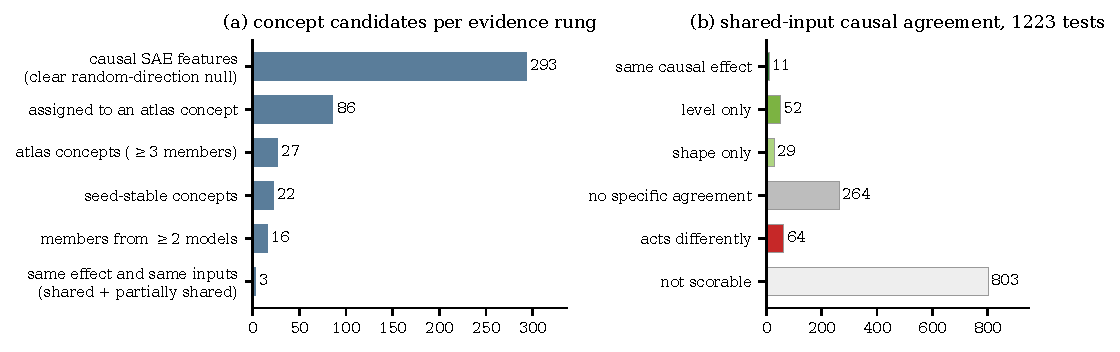
\includegraphics[width=\textwidth]{figures/funnel.pdf}
\caption{(a) Concept candidates at each rung (the first three bars are sequential; the last three are properties of the
11 atlas concepts). (b) Shared-input causal agreement over 1{,}290 tests drawn from the 1{,}296 reciprocal transfers.
Source: \texttt{sae/concept\_stage.json}.}
\label{fig:funnel}
\end{figure}

\subsection{RQ3: Do concepts causally affect the forecast?}
\label{sec:rq3}

\textbf{Answer.} Single features do causally shape the forecast, and some effects replicate on new series at the
attainable significance floor. The effects are small, fewer than half replicate, and neither activation prominence nor
attention mass identifies them.

\paragraph{Single-feature effects replicate partially.} Of 31 testable single-feature causal claims registered from v2
dev, 10 confirm on the private split, each with $p=0.001$ after an adaptive redraw to 1{,}000 null draws and
$p_{\text{Holm}}=0.031$, the floor for 31 tests. The confirmed share is highest for TimesFM (3 of 4) and lowest for
Chronos-2 (1 of 7) and Chronos-T5-Base (0 of 4); by channel, near-horizon shape (4 of 8), MASE (3 of 8) and spectral
centroid (2 of 4) confirm most often. Of the 21 claims not detected, 19 had not reached the 200-draw $p$ floor on dev. On
v3, under the stricter null, 11 of 24 claims confirm.

\paragraph{Activation prominence does not identify causal importance.} Of the 927 most prominent features of the private
atlas, 0.835 have no causal effect (one-sided lower bound 0.817; dev 0.810; $p_{\text{Holm}}=0.0005$; \fid{MN-14}); on v3
the share is 0.919 of 861. \tool{} therefore ranks features by measured effect rather than by activation.

\paragraph{The effects are small.} The median single-feature effect is 0.097 context standard deviations, 2.2 times
smaller than the 0.214 by which substituting the SAE reconstruction moves the forecast (v3: 0.156 against 0.260, 1.7
times; \fid{MN-15}). Among clearing cells, the median effect is 1.24 times the null's 95th percentile. The expressible
forecast change is nonetheless concentrated: zeroing the five attribution-ranked atoms of a layer produces a median 0.74
share of it, more than activation-matched random sets of five atoms on 30 of 31 targets (\fid{D-42C}).

\paragraph{Attention mass is not causal importance.} The attention mass a head places on seasonal lags is uncorrelated
with the seasonal power lost when the head is ablated ($\rho=0.026$ in TimesFM and $-0.118$ in Chronos-T5-Base;
\fid{CA-04}), consistent with \citet{jain2019attention}. A minimal seasonality circuit is one head in TimesFM but five
non-additive heads in Chronos-T5-Base (\fid{CA-03}).

\subsection{RQ4: Where in depth, and how comparable is depth?}
\label{sec:rq4}

\textbf{Answer.} How TimesFM and Chronos-2 react to corruptions across depth replicates for 6 of 9 corruptions on v2 and
4 of 9 on v3, with 8 of 9 keeping their sign. Absolute depth locations are comparable only after accounting for captured
compute.

\paragraph{Depth-resolved reaction profiles replicate.} The rank correlation between the two models' per-layer corruption
fingerprints replicates on the v2 private split for 6 of 9 corruptions (overall $\rho=0.524$ [0.504, 0.544];
Figure~\ref{fig:heldout}a). They react at matching depths to detrending (private $\rho=0.368$) and dropout (0.510), at
opposite depths to noise ($-0.743$), spikes ($-0.785$) and warps ($-0.651$), and not systematically to deseasonalizing
(0.086 [$-0.027$, 0.186]). Of the three that miss the registered rule (dev value inside the private interval), frequency
shift (0.381 against 0.216 on dev) and smoothing ($-0.581$ against $-0.418$) are \emph{stronger} on private data, while
level shift changes sign (dev $-0.188$; private 0.109). On v3 level shift flips again (dev $-0.164$; private 0.252), the
one depth agreement that is not stable across corpora.

\paragraph{Where restoration happens.} In TimesFM, restoration by per-window patching concentrates in the window just
before the horizon and grows with depth, from 0.427 at layer 0 to 0.612 at layer 8 and 0.631 at layer 16 for the noise
corruption, while restoration in the first window falls from $-0.191$ to 0.000 (320 v2 series; \fid{DE-01}).

\paragraph{Depth locations need qualification.} Captured compute ranges from 13.9\% (Chronos-T5-Base) to 99.8\% (Timer)
of a forecast's FLOPs (\fid{DE-05}), and Chronos-T5's last encoder block sits at depth 0.478 on the whole-stack axis
(\fid{DE-04}); the report renders both next to every depth claim. No layer chosen by one of three layer selectors is
robust to the choice of selector for any model (\fid{DE-08}).

\subsection{Can internals predict forecast failure?}
\label{sec:practical}

For each model we predict a series' log MASE (Spearman) and a failure flag (AUROC) from free, output-only features
(quantile width, flatness, catch22 features of the context), add the SAE-family activations at the last window, and
measure the gain, cross-fitted with a series bootstrap on 941 dev series. The evidence class is \ev{predictive}. The free
baseline is strong (Spearman 0.76--0.85), and for five models the gain's interval includes zero for both tasks. The gain is
positive for the two least accurate models, Timer (+0.030 [0.019, 0.043]) and Time-MoE (+0.012 [0.005, 0.019]); both
were registered and confirm when the frozen procedure is refit on the private split ($n=935$): Timer 0.0446 [0.0292,
0.0605], $p_{\text{Holm}}=0.002$, Time-MoE 0.011 [0.0032, 0.0194], $p_{\text{Holm}}=0.012$, and again on v3 (\fid{MN-28}).
Internals do not help choose a model: routing each series to the model with the lowest predicted MASE gives 1.964
[1.837, 2.093] with internals against 1.948 [1.814, 2.070] without ($p=0.258$), both worse than always using Chronos-2
(1.856).

\begin{table}[!tb]
\centering
\footnotesize
\setlength{\tabcolsep}{3pt}
\scriptsize
\begin{tabularx}{\textwidth}{@{}l>{\raggedright}Xllll@{}}
\toprule
RQ & Result (v2 unless stated) & Evidence class & Status & ID \\
\midrule
1 & 442 feature-channel cells clear an isotropic null, 2.47$\times$ empirical chance; Timer 1.02$\times$ & causal within-model & exploratory & MP-07, PM-17 \\
1 & Against an on-manifold null, features exceed chance only modestly (v3: 91 vs.\ 70.4, 1.29$\times$) & causal within-model & exploratory & CA-12 \\
1 & 79 of 91 v3 causal features clear under mean, resample or clean ablation; 37 under all three & causal within-model & exploratory & MP-10 \\
1 & 9 families cover 99\% of features but do not beat a shuffle null ($p=0.68$) & descriptive & exploratory & CA-10 \\
2 & All 21 pairs above null with concatenated windows; TimesFM/Chronos-2 0.712 dev, 0.707 fresh private; the window mean understates it by 0.30--0.43 & geometric & held-out confirmed & SH-01, MN-38 \\
2 & 7 similarity metrics agree only weakly ($W=0.25$) & mixed & exploratory & SH-05/06 \\
2 & Concept transfer on inputs: 20/20 on v2 and v3, 20/20 on raw real windows & correlational & held-out confirmed (2 corpora) & SH-18 \\
2 & Level and seasonality-damping causal features in all 7 models & descriptive & exploratory & CA-10 \\
2 & No concept spans more than 3 of 7 models & descriptive & held-out confirmed (2 corpora) & SH-16 \\
2 & Same effect on same inputs: 7/216 scorable, all Chronos-2/Bolt; test specific (0/9 decoys) & causal on shared inputs & exploratory & SH-22, MN-30 \\
2 & Multi-model atlas concepts 0/3; shared-input agreement 0/6 & causal, compared & not confirmed & CA-11 \\
3 & Single-feature causal effects: 10/31; v3 11/24 & causal within-model & partly confirmed & CA-11/12 \\
3 & 83.5\% of prominent features causally null (927 held-out; v3 91.9\%) & causal within-model & held-out confirmed & MN-14 \\
3 & Feature effect 2.2$\times$ below SAE reconstruction cost (v3 1.7$\times$) & causal within-model & exploratory & MN-15 \\
3 & Attention mass uncorrelated with head causality & causal vs.\ descriptive & exploratory & CA-04 \\
4 & Depth-profile agreement 6/9 corruptions; v3 4/9; level shift flips on both & causal within-model & partly confirmed & CA-01 \\
-- & Internals predict failure for the two weakest models only & predictive & held-out confirmed (2 corpora) & MN-28 \\
-- & Chronos-2 more accurate than TimesFM on \texttt{mixture} (0.209; v3 0.303) & behavioral & held-out confirmed (2 corpora) & PM-05 \\
\bottomrule
\end{tabularx}
\caption{Headline results with evidence class and status. Each ID is an entry in \repo{FINDINGS.md} with exact numbers, reproduction command and artifact path.}
\label{tab:results}
\end{table}
